\chapter{Final Project}

In this project we will configure a network combining the different technologies that we have learned along the course.
We will extend the topology in the routing assignment with wireless connectivity (WLAN) and security (Firewalls,IPSec) and traffic monitoring (Wireshark).

\section{Topology}

The topology that we will construct is presented in Fig. \ref{fig:final-topology}.
As in the routing assignments, each group will configure a part of the topology.
In this assignment, each group will take care of a router, a firewall, a switch, an access point and the necessary PCs.
This topology interconnects secured networks (behind a firewall) with another network that offers access to the Internet.
Each secured network needs at least a PC and an FTP server.

\begin{figure}
\centering
\ifpdf
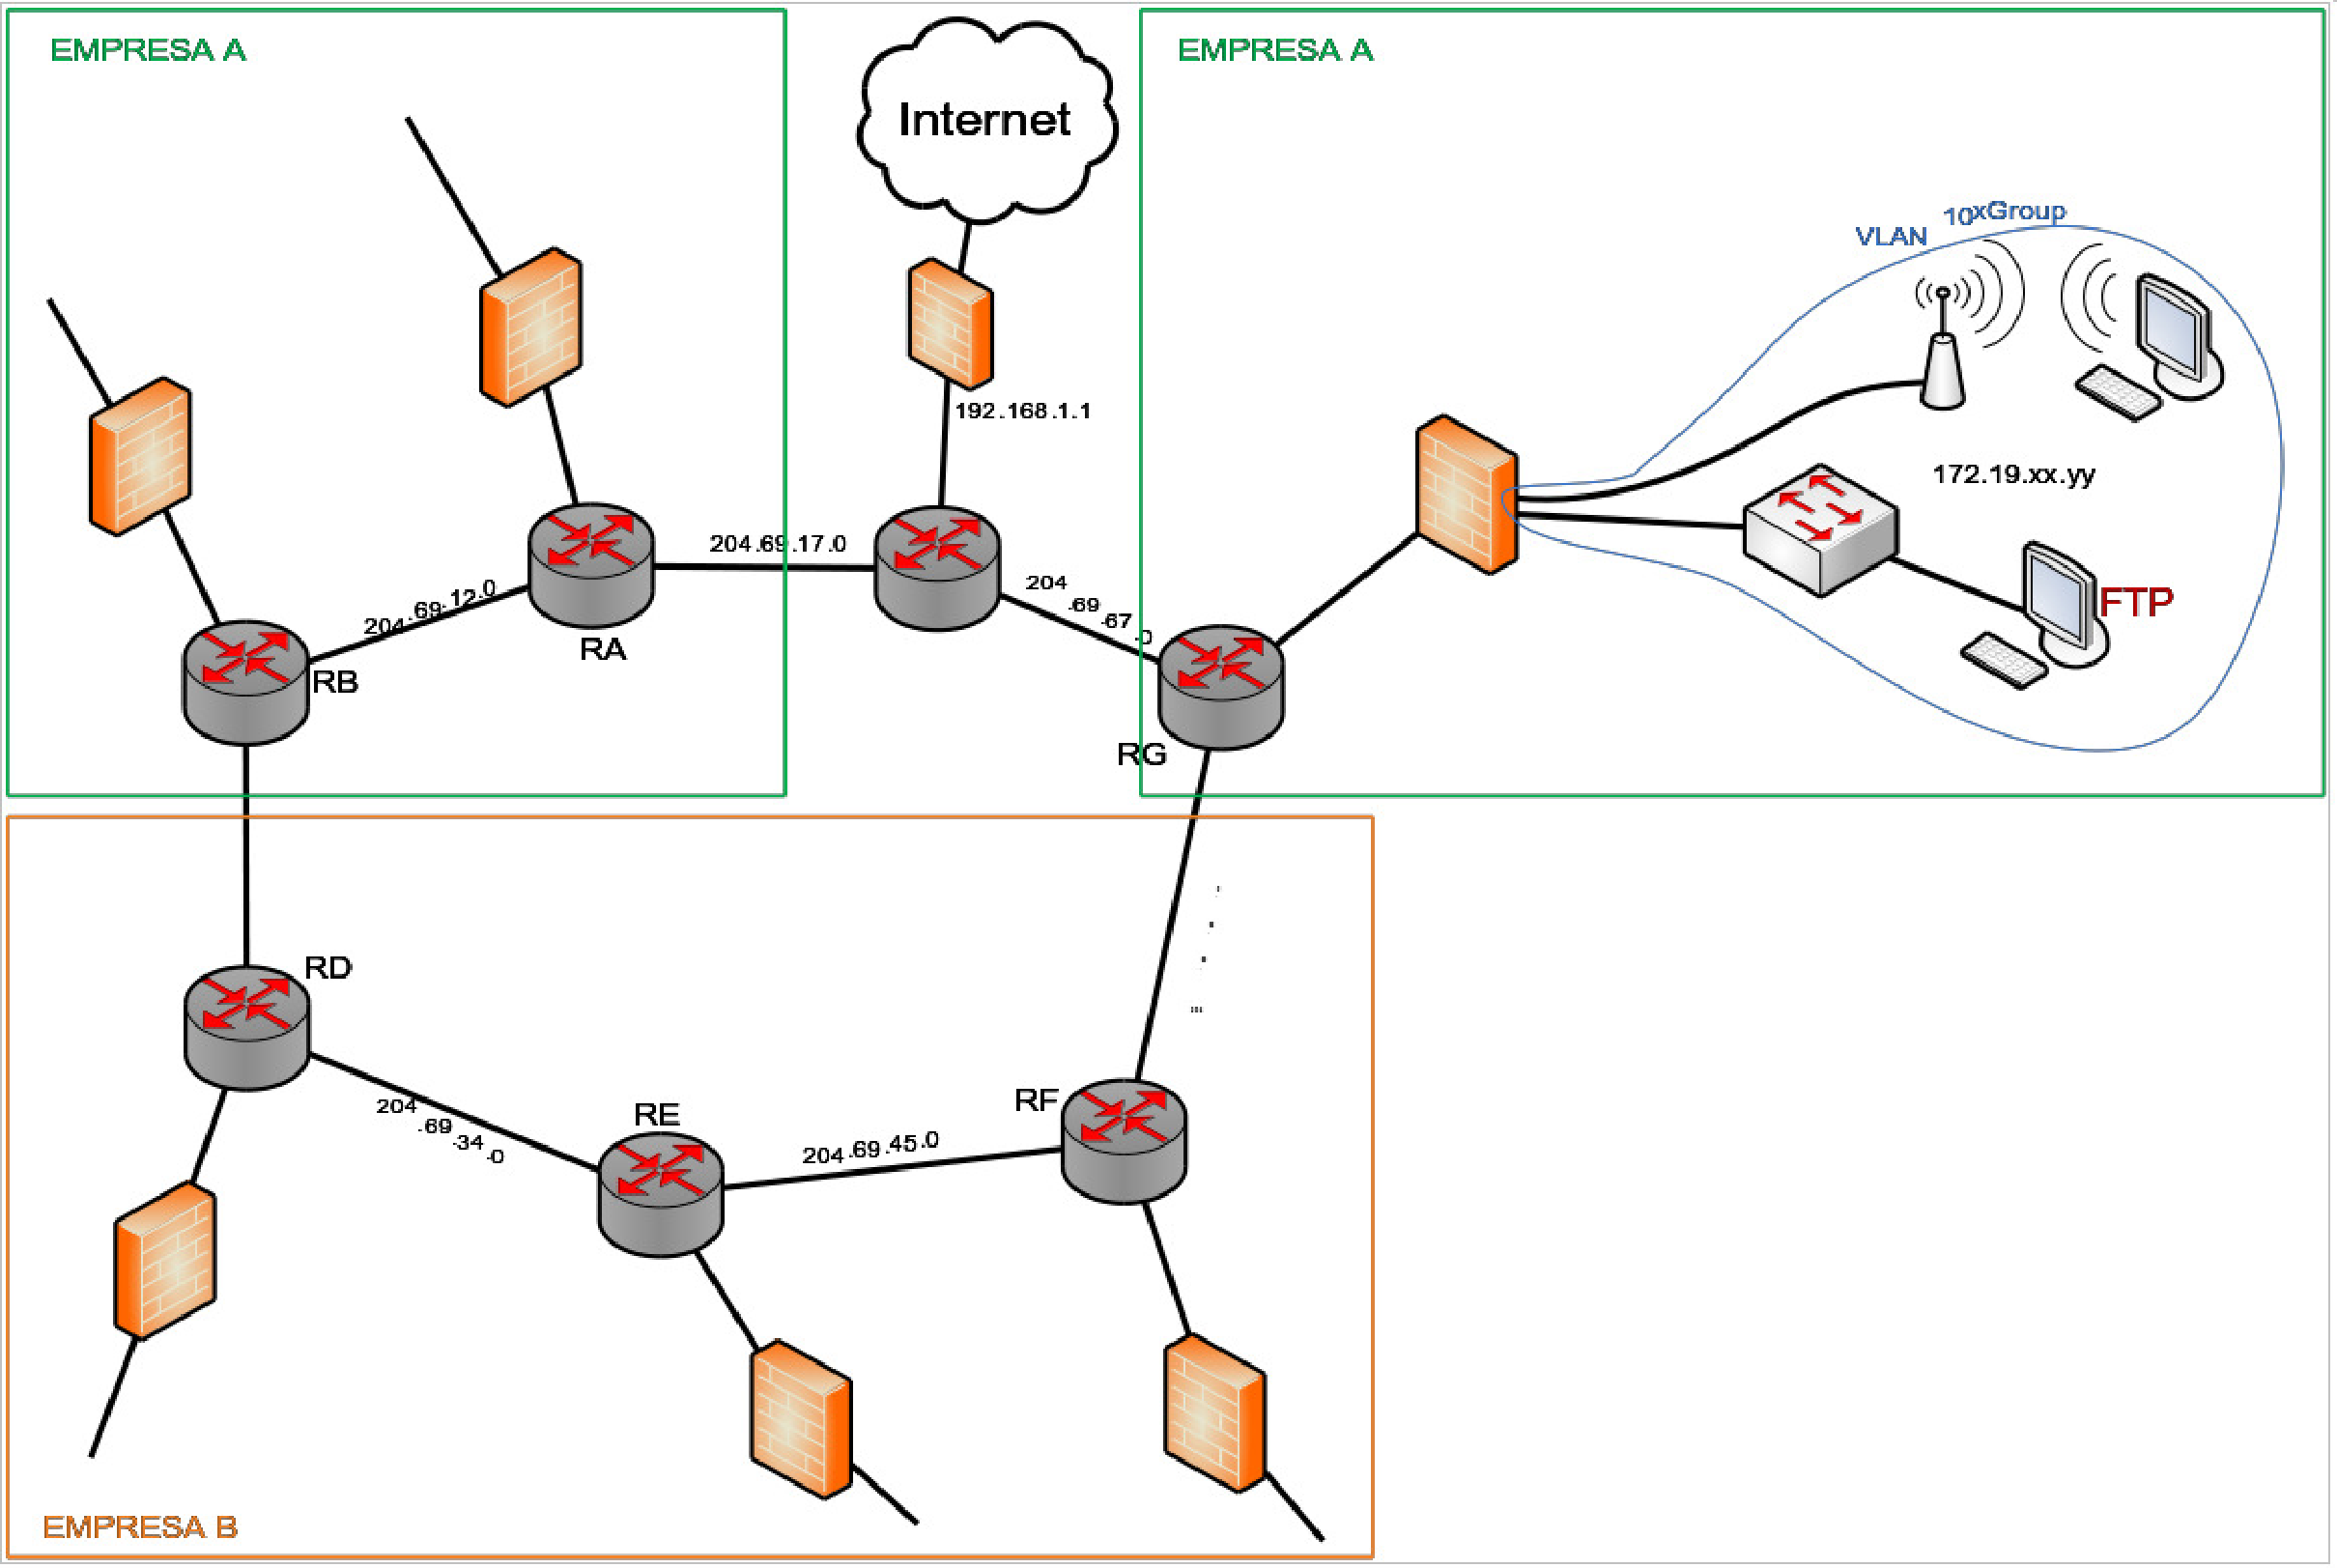
\includegraphics[width=0.9\linewidth]{Figures/final-topology.pdf}
\else
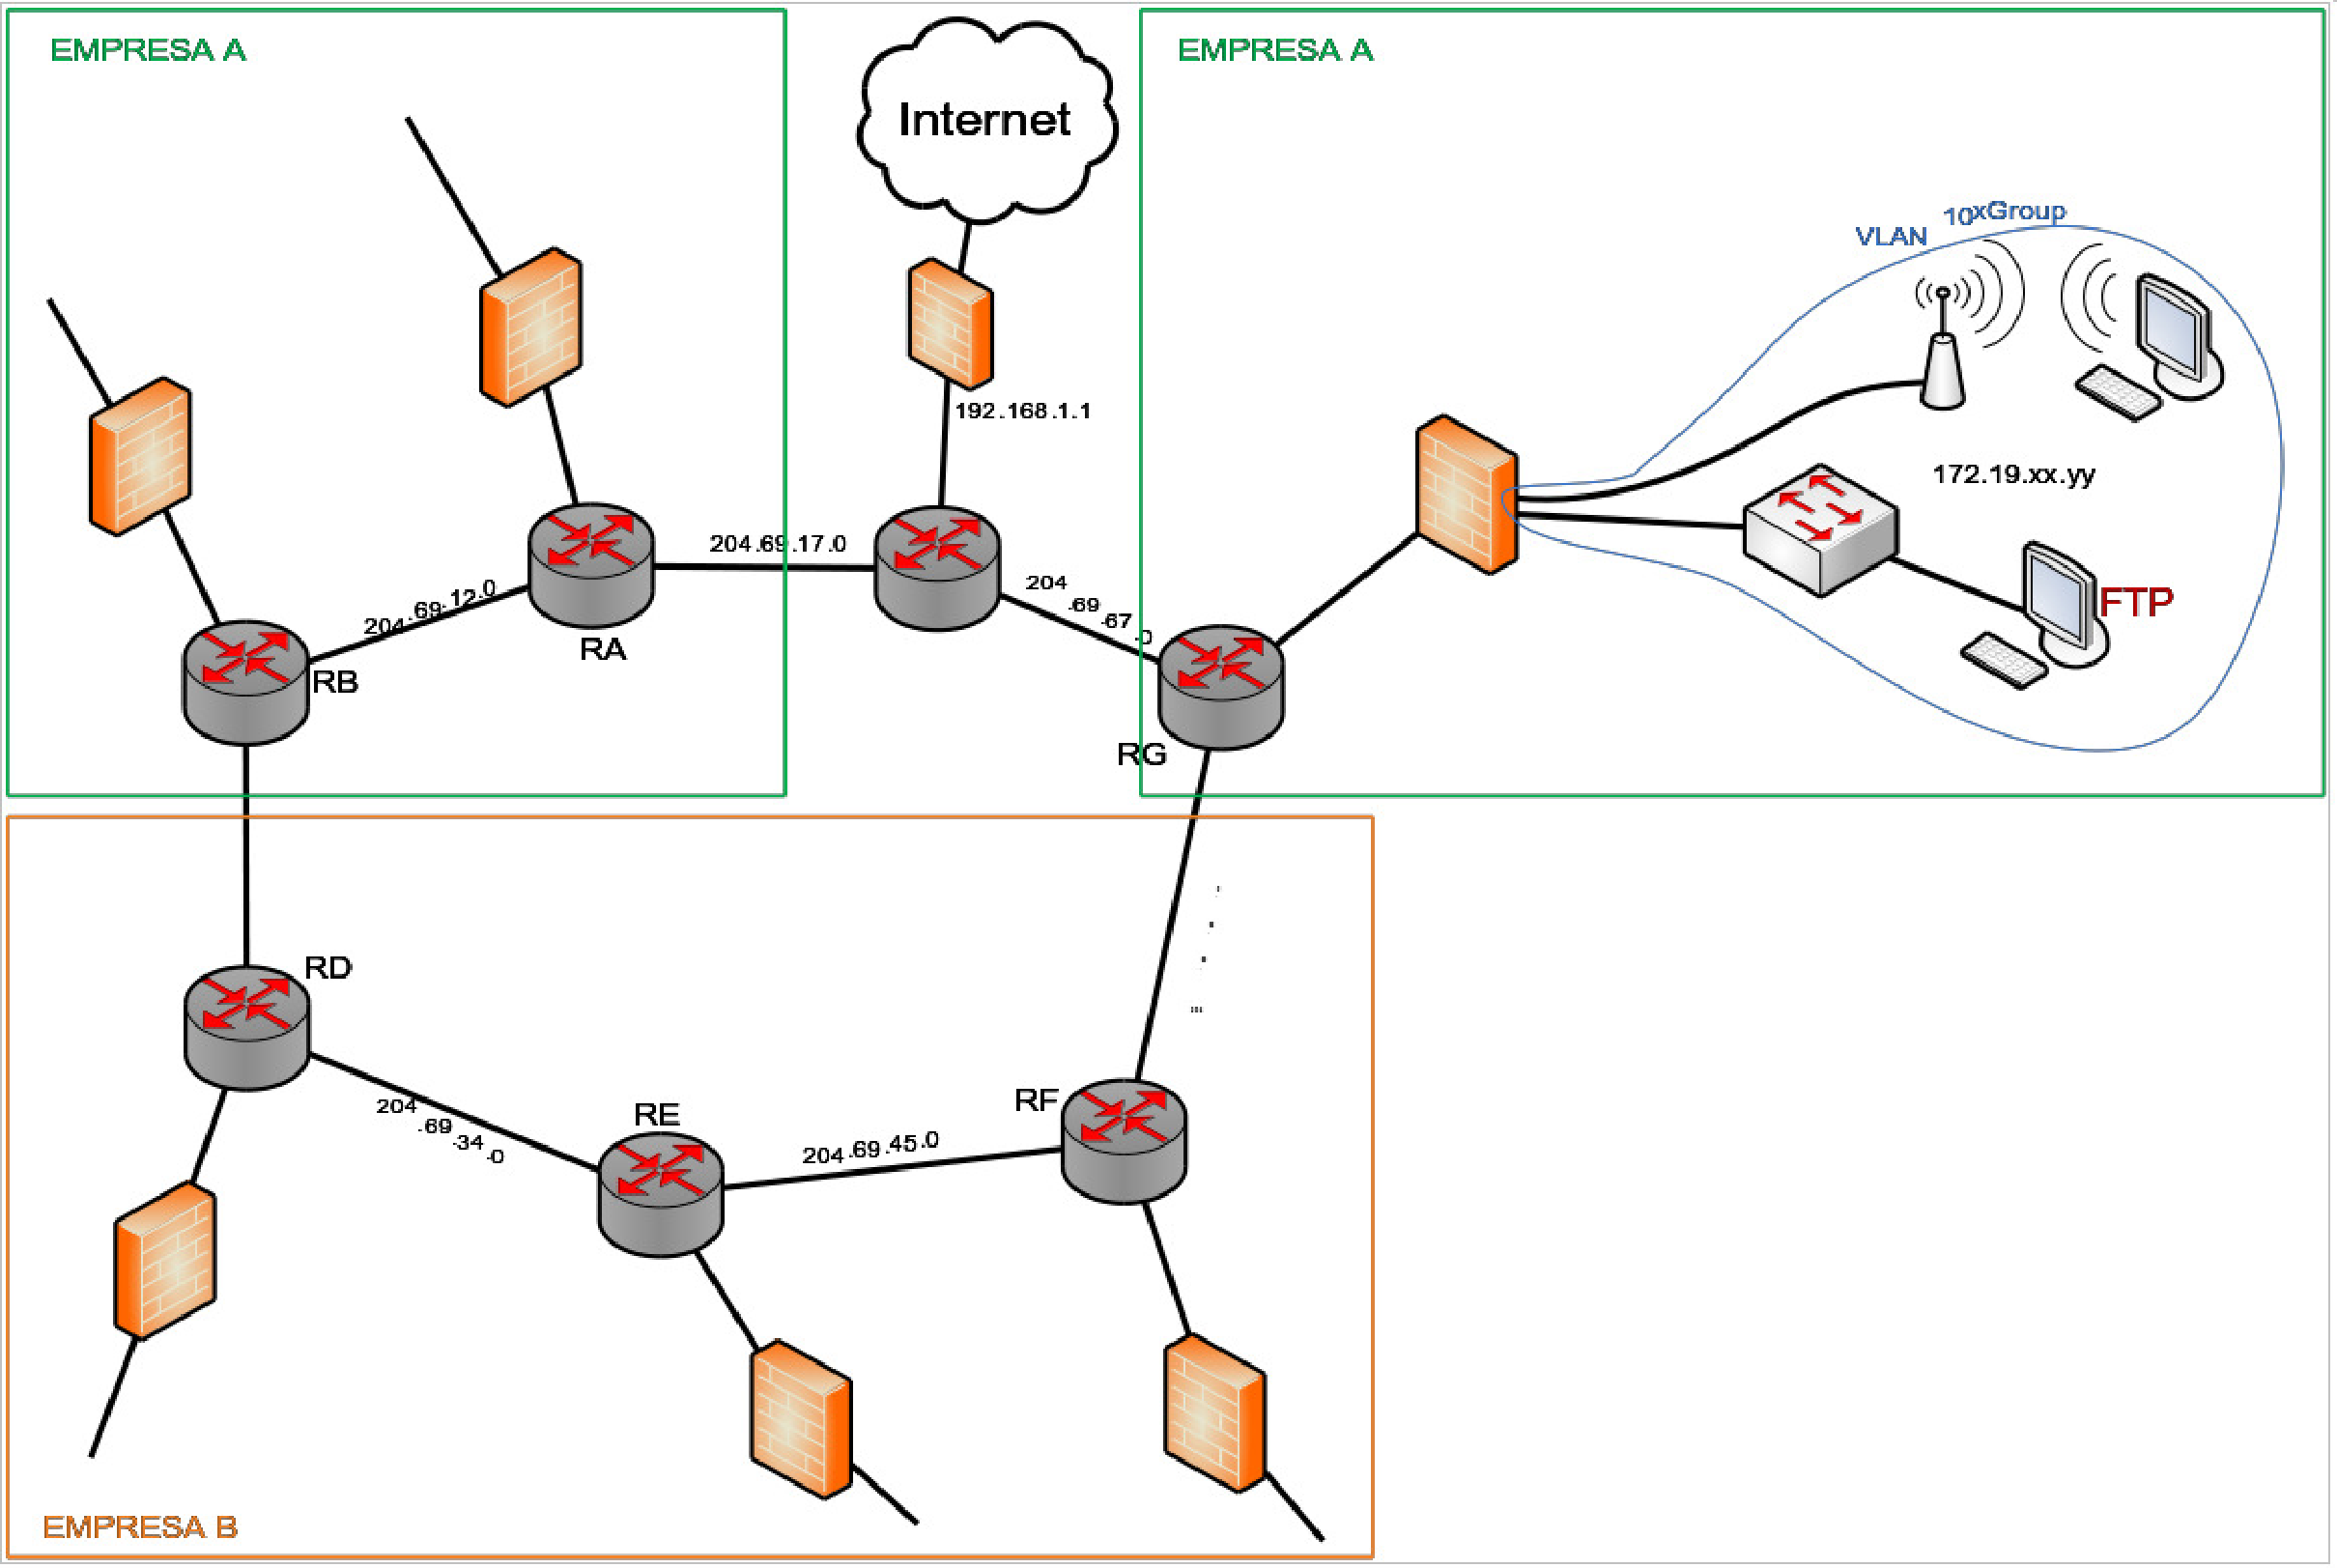
\includegraphics[width=0.9\linewidth]{Figures/final-topology.eps}
\fi
\caption{Topology of the final assignment}
\label{fig:final-topology}
\end{figure}

\section{Equipment and addresses}
The assignment of equipment and addresses to the groups is detailed in Table~\ref{tab:equipment-and-addresses}.
The switches are shared and the table specifies the ports for each group.
The IP addresses for WiFi devices, Ethernet devices, the FW interior interface and the public addresses are also included.

Note that the in the interior networks we use a 23 bits netmask.
This means that both WiFi stations and Ethernet stations are in fact in the same subnet.

For the serial links with public addresses between routers 
\begin{table}
\sffamily\small
\centering
\begin{tabular}{cccccccc}
\hline
Group & Router & Switch & Ports & IPs WiFi & IPs Eth & FWin & IPs public \\
\hline
1 & A & B & 1-6 & .80.1X/23 & .81.1X/23 & .80.1/23 & 201.69.10.0/24 \\
2 & B & B & 7-12 & .82.1X/23 & .83.1X/23 & .82.1/23 & 201.69.20.0/24 \\
3 & D & C & 1-6 & .84.1X/23 & .85.1X/23 & .84.1/23 & 201.69.30.0/24 \\
4 & E & C & 7-12 & .86.1X/23 & .87.1X/23 & .86.1/23 & 201.69.40.0/24 \\
5 & F & D & 1-6 & .88.1X/23 & .89.1X/23 & .88.1/23 & 201.69.50.0/24 \\
6 & G & D & 7-12 & .90.1X/23 & .91.1X/23 & .90.1/23 & 201.69.60.0/24 \\

\end{tabular}
\caption{Equipment and addresses}
\label{tab:equipment-and-addresses}
\end{table}

\section{Security guidelines}
We will imagine that each team is configuring a company site.
There will be two companies and three sites per company.
The security guidelines are as follows:
\begin{itemize}
\item The internal PCs should be able to connect to the internal FTP server.
\item The PCs of other sites of the same company should be able to connect to our FTP server.
\item The PCs of sites of the other company should not be able to connect to our FTP server.
\item Our PCs should be able to ping outer hosts.
\item It should not be possible for outer PCs to ping our hosts.
\item PCs should have Internet connectivity.
\end{itemize}

\section{Device configuration}
We have to configure the devices in our site:
\begin{itemize}
\item Switch: Creating the VLANs and assigning ports.
\item Router: Serial and ethernet interfaces. Routing protocol.
\item AP: Basic configuration.
\item Firewall: NAT translation, filtering rules, inside and outside interface.
\end{itemize}

To configure the switch, you need to be connected to VLAN1.
To configure the router, you can use the console connection.
To configure the FW and the AP, you can directly connect to them.

\section{Home preparation}

Find which ranges of IP are private addresses.
Find information about Classless Inter-Domain Routing and what is the difference between /23 and /24.


\begin{center}
\sffamily\small
\begin{tabular}{>{\columncolor{tablegray}}p{15cm}}

\multicolumn{1}{>{\columncolor{tableorange}}l}{Questions}\\
Do the addresses assigned to WiFi and ethernet devices belong to the same subnet? Why?\\
What is the explanation for the IP address for the internal interface of the FW?\\
\hline
\end{tabular}
\end{center}

Fill in Fig.~\ref{fig:final-topology} with the configuration information (port, switch, IPs, NAT, firewall rules, etc.)

\section{Steps and checkpoints for device configuration}
\begin{itemize}
\item Step: Study the configuration.
\item Checkpoint: Complete the configuration information on the figure.
\item Step: Configure the switches (VLANs and ports).
\item Checkpoint: VLANs created and ports assigned.
\item Step: Configure the FW interfaces.
\item Checkpoint: Ping the FW from the PC.
\item Step: Configure the router (interfaces, RIP, routes, etc.)
\item Checkpoint: ping from the router to the firewall, ping between routers, routing table, ping between firewalls.
\item Configure the FW rules and NAT.
\end{itemize}

More details in Section~\ref{sec:final-tips}

\section{Lab report}

The lab report should include both the devices configuration and the validation tests.
As a minimum, it should contain:
\begin{itemize}
\item Complete network figure with all the IPs, VLANs, ports, etc.
\item Configuration
\begin{itemize}
\item Routing tables.
\item NAT and filtering rules configuration.
\item Use the appendixes for snapshots.
\end{itemize}
\item Tables with results of the validation tests (connectivity, delay, throughput, etc.)
\end{itemize}

\section{Optional assignments}
Configure the firewall to prevent that wireless stations connect to the FTP server.
Create a VPN between the sites of the company.

\section{Final tips}
\label{sec:final-tips}

The IPs of the switches are:
\begin{itemize}
\item A: 192.168.1.111
\item C: 192.168.1.112
\item D: 192.168.1.113
\end{itemize}

The DNS of the upf is 193.145.56.11

\subsection{Firewall configuration}
j
\begin{itemize}
\item Connect the PC to the FW (inside)
\item Enable https access to the network 172.19.XX.0
\item Change the inside interface address to 172.19.XX.XX/23 . We will lose connectivity.
\item Change the IP of the PC to 172.19.XX.XX/23. Default gateway is the inside interface of the FW. Restart ASDM.
\item Change the external IP of the firewall to 204.69.XX.XX/24
\item Add a static default route at the outside interface of the FW. 0.0.0.0-0.0.0.0 with the router interface as a gateway.
\end{itemize}

\subsection{Router configuration}
\begin{itemize}
\item Configure the IP of the ethernet interface.
\item Configure the IP of the serial interfaces. 204.69.XX.XX/24 clockrate ~ 200.000
\item Add RIP to the routers. Add all networks. Check routing table.
\item Configure Internet access. Add an static route to the gateway of the lab. ip route 0.0.0.0 0.0.0.0 192.168.1.1
\end{itemize}

\subsection{Access point configuration}
\begin{itemize}
\item Change the IP of the AP and set the FW as the default gateway. Use the console to change the IP address of the interface bvi1.
\item Make sure that HTTP access is enabled.
\item Connect the AP to the firewall.
\item Use a PC with wired connection and the browser to connect to the AP. Configure the gateway. Configure also the wireless network (SSID, broadcast, radio interface up).
\item Add a DHCP server to the FW to serve address to wireless PCs. Properties $\rightarrow$ DHCP $\rightarrow$ DHCP Server $\rightarrow$ Configure IP range and DNS.
\end{itemize}
